% ----- ----- ----- ----- ----- ----- ----- ----- ----- -----
% Preamble
% ----- ----- ----- ----- ----- ----- ----- ----- ----- -----
\documentclass[a4paper,9pt]{article}
\usepackage[utf8]{inputenc}
\usepackage[english]{babel}
\usepackage{amsmath}
\usepackage{authblk}
\usepackage{background}
\usepackage{enumitem}
\usepackage{fancyhdr}
\usepackage{geometry}
\usepackage{graphicx}
\usepackage[hidelinks]{hyperref}
\usepackage{indentfirst}
\usepackage{listings}
\usepackage{multicol}
\usepackage{tabularx}
\usepackage[most]{tcolorbox}
\usepackage{tgheros}
\usepackage[explicit]{titlesec}
\usepackage{xcolor}
% ----- ----- ----- ----- -----
% Column Spacing
% ----- ----- ----- ----- -----
\setlength{\columnseprule}{0pt}
\setlength{\columnsep}{10.0pt}
\newcolumntype{L}[1]{>{\raggedright\let\newline\\\arraybackslash\hspace{0pt}}m{#1}}
\newcolumntype{C}[1]{>{\centering\let\newline\\\arraybackslash\hspace{0pt}}m{#1}}
\newcolumntype{R}[1]{>{\raggedleft\let\newline\\\arraybackslash\hspace{0pt}}m{#1}}
% ----- ----- ----- ----- -----
% Custom Colors
% ----- ----- ----- ----- -----
\definecolor{myDColor}{HTML}{000000} % Darker Color
\definecolor{myLColor}{HTML}{CFB87C} % Lighter Color
\definecolor{LinkColor}{HTML}{CFB87C} % Link Color
% ----- ----- ----- ----- -----
% Custom Title
% ----- ----- ----- ----- -----
\makeatletter
\renewcommand*{\maketitle}{%
\noindent
\begin{minipage}{\textwidth}

\begin{tikzpicture}
\node[rectangle,rounded corners=10pt,inner sep=7.5pt,fill=myDColor,text width= 0.975\textwidth, align=center]
{\color{white}\Huge \@title};
\end{tikzpicture}
\end{minipage}
\hfill
\bigskip\bigskip
}%
\makeatother
% ----- ----- ----- ----- -----
% Custom Section
% ----- ----- ----- ----- -----
\newcommand*\sectionlabel{}
\titleformat{\section}
{\gdef\sectionlabel{}
\normalfont\sffamily\Large\bfseries\scshape}
{\gdef\sectionlabel{\thesection\ }}{0pt}{
\noindent
\begin{tikzpicture}
\node[rectangle,rounded corners=6pt,inner sep=4pt,fill=myLColor,text width= 0.975\columnwidth, align=center]
{\color{white}\sectionlabel#1};
\end{tikzpicture}}
\titlespacing*{\section}{0pt}{5pt}{5pt}
% ----- ----- ----- ----- -----
% Custom Header & Footer / Geometry
% ----- ----- ----- ----- -----
\geometry{a4paper,left=10mm,right=10mm,top=15mm,bottom=15mm}
\linespread{1} % Distance between lines
\pagestyle{fancy}
\fancyhead[L]{Taylor Larrechea}
\fancyhead[C]{Exam 1 Study Guide}
\fancyhead[R]{University of Colorado}
\fancyfoot[L]{CSPB 2270 Data Structures}
\fancyfoot[R]{Exam 1 Study Guide}
\backgroundsetup{
    scale = 1,
    angle = 0,
    opacity = 0.1,
    contents = {
    
\includegraphics[scale = 0.25, keepaspectratio]{Figures/CU Seal.png}
    }
}
\newtcolorbox{highlight}[1][]{%
    enhanced,
    skin first=enhanced,
    skin middle=enhanced,
    skin last=enhanced,
    before upper={\parindent15pt},
    breakable,
    boxrule = 0pt,
    frame hidden,
    borderline west = {4pt}{0pt}{myDColor},
    colback = myLColor!10,
    coltitle = myLColor!5,
    sharp corners,
    rounded corners = southeast,
    arc is angular,
    arc = 3mm,
    attach boxed title to top left,
    boxed title style = {%
        enhanced,
        colback = myDColor,
        colframe = myDColor,
        top = 0pt,
        bottom = 0pt,
        sharp corners,
        rounded corners = northeast,
        arc is angular,
        arc = 2mm,
        rightrule = 0pt,
        bottomrule = 0pt,
        toprule = 0pt,
    },
    title = {\bfseries\large #1},
    overlay unbroken={%
        \path[fill = tcbcolback!80!black]
            ([yshift = 3mm]interior.south east) -- ++(-0.4,-0.1) -- ++(0.1,-0.2);
    },
    overlay first = {%
        \path[fill = tcbcolback!80!black]
            ([yshift = 3mm]interior.south east) -- ++(-0.4,-0.1) -- ++(0.1,-0.2);
    },
    overlay middle={%
        \path[fill = tcbcolback!80!black]
            ([yshift = -3mm]interior.north east) -- ++(-0.4,0.1) -- ++(0.1,0.2);
        \path[fill = tcbcolback!80!black]
            ([yshift = 3mm]interior.south east) -- ++(-0.4,-0.1) -- ++(0.1,-0.2);
    },
    overlay last={%
        \path[fill = tcbcolback!80!black]
            ([yshift = -3mm]interior.north east) -- ++(-0.4,0.1) -- ++(0.1,0.2);
        \path[fill = tcbcolback!80!black]
            ([yshift = 3mm]interior.south east) -- ++(-0.4,-0.1) -- ++(0.1,-0.2);
    },
    extras middle and last = { rounded corners = northeast }
}
\newcommand{\horizontalline}{\noindent \rule{\textwidth}{0.5pt}}
\newcommand{\function}[1]{\textbf{#1}}
\lstnewenvironment{code}{\horizontalline \vspace{-0.5em} \lstset{basicstyle=\ttfamily}}{\vspace{-1em} \horizontalline}
% ----- ----- ----- ----- ----- Title
\title{CSPB 2270 Exam 1 Study Guide}
% ----- ----- ----- ----- ----- Begin Document
\begin{document}

\maketitle

\section*{Binary Search Trees}

\subsection*{Overview}

Binary Search Trees (BSTs) are a type of binary tree data structure that maintain a specific order of elements. In a BST, each node has a key or value, and the keys of nodes in the left subtree are 
less than the key of the current node, while the keys of nodes in the right subtree are greater. This property enables efficient searching, insertion, and deletion operations. BSTs offer fast average 
case performance for these operations, with a time complexity of $\mathcal{O}(\log{(n)})$ in balanced trees. They are commonly used in scenarios that require fast searching or ordered traversal of elements, 
such as dictionary implementations, range queries, and efficient data organization.

A Binary Search Tree (BST) and a linked list differ in their structure and organization of data. A BST is a binary tree where nodes are ordered based on their keys, allowing for efficient search, insertion, 
and deletion operations. In contrast, a linked list is a linear structure where elements are connected via pointers, without a specific ordering. Traversing a linked list requires sequentially following the 
next pointers, while a BST enables faster search and manipulation of elements due to its ordered nature.

A balanced tree is a tree data structure in which the heights of the left and right subtrees of any node differ by at most one. It ensures that the tree is evenly balanced and maintains efficient operations. 
Balanced trees are desirable because they provide improved performance for various operations such as searching, inserting, and deleting elements. By keeping the tree balanced, the height remains relatively 
low, which reduces the time complexity of operations and ensures that the worst-case scenario is avoided. Common examples of balanced trees include AVL trees, red-black trees, and B-trees.

BST's have some common terminology that are useful to describe certain aspects of the structure. The terminology that we use to describe a BST can be seen below:

\begin{itemize}
    \item \textbf{Children:} Children are defined as nodes that are connected to a parent node, either left or right, in the hierarchical structure of the tree
    \item \textbf{Complete:} A BST where if all levels, except the last level, contain all possible nodes and all nodes in the last level are as far left as possible
    \item \textbf{Depth:} Depth is defined as the number of edges on the path from the root to the node in question
    \item \textbf{Edge:} An edge is a link from a parent node to its child node
    \item \textbf{Full:} A BST where every node contains 0 or 2 children
    \item \textbf{Height:} The height of a tree is the largest depth of any node in the tree
    \item \textbf{Internal Node:} An internal node is a node with at least one child
    \item \textbf{Leaf:} A leaf is a node with no children
    \item \textbf{Level:} The level of a BST is defined as nodes that have the same depth
    \item \textbf{Parent:} A parent is a node where one of more child nodes are directly connected to it
    \item \textbf{Perfect:} A BST where if all internal nodes have 2 children and all leaf nodes are at the same level
    \item \textbf{Root:} The root of a BST is referred to as the topmost node of the tree structure (The root node has no parent node)
\end{itemize}

\noindent The terms: \textbf{Full}, \textbf{Complete}, and \textbf{Perfect} define special types of BST's. The rest of the terms in the above list are components of the BST

BST's use a technique called recursion. Recursion is a programming technique where a function calls itself to solve a smaller instance of the same problem. It is useful in dealing with trees because trees are 
recursive data structures. Each node in a tree can be viewed as a smaller tree itself, consisting of its children and their descendants. Recursion allows us to traverse and manipulate tree structures by breaking 
down the problem into smaller sub problems that can be solved recursively. It simplifies the code by abstracting the complex tree operations into simpler recursive calls, leading to concise and elegant solutions. 
Additionally, recursion provides a natural way to handle tree-related algorithms, such as tree traversal, searching, insertion, deletion, and various other tree-based computations.

\subsection*{Common BST Operations}

BST's require a number of operations for the functionality of it to be optimal. A lot of these operations can also be seen in linked lists. The operations that are used in BST's are the following:

\begin{itemize}
    \item \textbf{Contains:} The contains function in a Binary Search Tree (BST) is used to check if a given value is present in the tree.
    \item \textbf{Get Node:} The getnode function in a Binary Search Tree (BST) is used to search for a node with a specified value in a tree.
    \item \textbf{Height:} The height operation in a BST recursively calculates the maximum number of edges from the root to any leaf node, providing a measure of the tree's vertical depth.
    \item \textbf{Initialize:} Initializing a node in a Binary Search Tree (BST) means creating a new node with a given value and setting its left and right child pointers to null or nullptr, indicating an empty subtree.
    \item \textbf{Insert:} The insert function in a Binary Search Tree (BST) is responsible for adding a new node to the tree while maintaining the binary search property, where values smaller than the current node are 
    placed in the left subtree, and values larger than the current node are placed in the right subtree.
    \item \textbf{In Order:} An in-order traversal function in a Binary Search Tree (BST) visits all the nodes in the tree in ascending order of their values.
    \item \textbf{Post Order:} A post-order traversal function in a Binary Search Tree (BST) visits all the nodes in the tree in a specific order.
    \item \textbf{Pre Order:} A pre-order traversal function in a Binary Search Tree (BST) visits all the nodes in the tree in a specific order.
    \item \textbf{Remove:} The remove function in a Binary Search Tree (BST) is used to delete a node from the tree while preserving the binary search property. It involves finding the node to be removed, handling different 
    cases based on the number of children the node has, and reorganizing the tree as necessary to maintain its structure and properties.
    \item \textbf{Size:} The size function in a Binary Search Tree (BST) is used to determine the number of nodes in a tree.
    \item \textbf{To Vector:} The tovector function in a Binary Search Tree (BST) is used to add values in a tree to a vector.
\end{itemize}

We can now look at each of these operations individually. The first operation that we will look at is the contains operation.

\begin{highlight}[Contains In BST]

\subsection*{Contains}

Below is an example of the implementation of the contains operation in a BST in the context of C++:

\begin{code}
bool BST::Contains(shared_ptr<bst_node> subt, int data){
    if (subt == nullptr) {
        return false;
    }
    else if (subt->data == data) {
        return true;
    }
    else {
        return Contains(subt->left, data) || Contains(subt->right, data);
    }
}
\end{code}

The above function takes in a node that is present in a BST and searches for a specific value in the list. It utilizes recursion to search both the left and right subtrees of the current node and
returns a boolean value determining if the value is present in the tree. The time complexity of this algorithm is the following: \newline

\begin{center}
    \begin{tabular}[ht]{|c|c|}
        \hline \textbf{Best Case Time Complexity} & \textbf{Worst Case Time Complexity} \\ \hline
        $\mathcal{O}(\log{(n)})$ & $\mathcal{O}(n)$ \\ \hline
    \end{tabular}
\end{center}

\noindent The best case time complexity occurs when the tree is balanced. The worst case time complexity occurs when the node doesn't exist or if the node is at the leaf level of the tree.

\end{highlight}

The next operation that we will look at is the GetNode operation.

\begin{highlight}[Get Node In BST]

\subsubsection*{Get Node}

Below is an example of the implementation of the Get Node operation in a BST in the context of C++:

\begin{code}
shared_ptr<bst_node> BST::GetNode(shared_ptr<bst_node> subt, int data){
    if (subt == nullptr) {
        return shared_ptr<bst_node>(nullptr);
    }
    else if (subt->data == data) {
        return subt;
    }
    else {
        if (GetNode(subt->left, data)) {
            return GetNode(subt->left, data);
        }
        else {
            return GetNode(subt->right, data);
        }
    }
}
\end{code}

This operation searches a BST for a specific value and returns the node if it exists. Similar to the contains operation the GetNode operation uitlizes recursion to search the left and right subtrees
of the node that is fed into the function. The time complexity of this algorithm is the following: \newline

\begin{center}
    \begin{tabular}[ht]{|c|c|}
        \hline \textbf{Best Case Time Complexity} & \textbf{Worst Case Time Complexity} \\ \hline
        $\mathcal{O}(\log{(n)})$ & $\mathcal{O}(n)$ \\ \hline
    \end{tabular}
\end{center}

\noindent The time complexity of this operation is the same as that of the operation that just searches for a value in a BST. When searching for the maximum or minimum value in a tree, the time complexity
is the same for searching for a value in the tree. These time complexities are contingent upon the balancing of the tree.

\end{highlight}

The next operation that we will look at is the Height operation.

\begin{highlight}[Height In BST]

\subsubsection*{Height}

Below is an example of the implementation of calculating the height of a BST in the context of C++:

\begin{code}
int height(Node* root) {
    if (root == nullptr) {
        return 0;  // An empty tree has height 0
    }
    else {
        // Recursively calculate the height of the left and right subtrees
        int leftHeight = height(root->left);
        int rightHeight = height(root->right);

        // Return the maximum height between the left and right subtrees, 
        // plus 1 for the current node
        return std::max(leftHeight, rightHeight) + 1;
    }
}    
\end{code}

\noindent The above function calculates the max number of edges to the leaf level in a BST. This function utilizes the concept of recursion to find which subtree has the most edges in it. This in turn is the
height of the BST.

\end{highlight}

The next operation that we will look at is the Initialize operation.

\begin{highlight}[Initializing In BST]

\subsubsection*{Initializing}

Below is an example of the implementation of initializing a node in a BST in the context of C++:

\begin{code}
shared_ptr<bst_node> BST::InitNode(int data){
    shared_ptr<bst_node> ret(new bst_node());
    ret->data = data;
    ret->left = nullptr;
    ret->right = nullptr;
    return ret;
}
\end{code}

The above function initializes a node for a BST. It sets the value of the 'data' member to the input parameter that is passed in the function. This operation has a constant time complexity of 
$\mathcal{O}(1)$.

\end{highlight}

The next operation that we will look at is the insert operation.

\begin{highlight}[Inserting In BST]

\subsubsection*{Inserting}

Below is an example of the implementation of inserting into a BST in the context of C++:

\begin{code}
void BST::Insert(shared_ptr<bst_node> new_node){
    if (GetRoot() == nullptr) {
        SetRoot(new_node);
    }
    else {
        shared_ptr<bst_node> current_node = GetRoot();
        while (current_node != nullptr) {
            if (new_node->data < current_node->data) {
                if (current_node->left == nullptr) {
                    current_node->left = new_node;
                    current_node = nullptr;
                }
                else {
                    current_node = current_node->left;
                }
            }
            else {
                if (current_node->right == nullptr) {
                    current_node->right = new_node;
                    current_node = nullptr;
                }
                else {
                    current_node = current_node->right;
                }
            }
        }
    }
}
\end{code}

The insert operation inserts a node into a BST in the correct spot in the tree. This function operates by searching through a BST for where the node should be inserted. Similar to that of the search
operation, the insert operation as the following time complexities: \newline

\begin{center}
    \begin{tabular}[ht]{|c|c|}
        \hline \textbf{Best Case Time Complexity} & \textbf{Worst Case Time Complexity} \\ \hline
        $\mathcal{O}(\log{(n)})$ & $\mathcal{O}(n)$ \\ \hline
    \end{tabular}
\end{center}

\noindent The time complexities of this operation are again contingent upon the balancing of the tree. This operation effecitvely searches through the BST to try and find the appropriate spot for where
it should be inserted. The best case scenario for inserting into a BST occurs when it is balanced and the worst case happens when the insertion happens at the leaf level.

\end{highlight}

The next operation that we will look at is the in order traversal of a BST.

\begin{highlight}[In Order Traversal In BST]

\subsubsection*{In Order}

Below is an example of the implementation of the in-order traversal of a BST in the context of C++:

\begin{code}
shared_ptr<bst_node> BST::InOrder(shared_ptr<bst_node> subt) {
    if (subt == nullptr) {
        return subt;
    }
    else {
        if (InOrder(subt->left)) {
            return InOrder(subt->left);
        }
        else {
            return InOrder(subt->right);
        }
    }
}
\end{code}

\noindent This function traverses a BST in order, meaning in ascending order. This function utilizes recursion to traverse the tree. It traverses in ascending order by traversing through all of the
left subtrees and then the right subtrees. The time complexity of the in order traversal is $\mathcal{O}(n)$ regardless of the balancing of the tree.

\end{highlight}

The next operation that we will look at is the post order traversal of a BST.

\begin{highlight}[Post Order Traversal In BST]

\subsubsection*{Post Order}

Below is an example of the implementation of post order traversal in a BST in the context of C++:

\begin{code}
void postOrderTraversal(shared_ptr<bst_node> root) {
    if (root == nullptr) {
        return;
    }
    
    // Visit the left subtree
    postOrderTraversal(root->left);
    
    // Visit the right subtree
    postOrderTraversal(root->right);
    
    // Process the root node
    std::cout << root->data << " ";
}    
\end{code}

\noindent The above function traverses a BST in post order fashion. In post-order traversal, the nodes of the BST are visited in the following order: left subtree, right subtree, and then the root. 
The recursive function is called first for the left subtree, then for the right subtree, and finally the root node is processed. Similar to the in order traversal, the time complexity of this operation
is $\mathcal{O}(n)$ regardless of the balancing of the tree.

\end{highlight}

The next operation that we will look at is the pre order traversal of a BST.

\begin{highlight}[Pre Order Traversal In BST]

\subsubsection*{Pre Order}

Below is an example of the implementation of pre order traversal in a BST in the context of C++:

\begin{code}
void PreOrderTraversal(std::shared_ptr<bst_node> root) {
    if (root == nullptr)
        return;

    // Process current node (root)
    std::cout << root->data << " ";

    // Recursively traverse left subtree
    PreOrderTraversal(root->left);

    // Recursively traverse right subtree
    PreOrderTraversal(root->right);
}
\end{code}

\noindent The above function traverse a BST in a pre order fashion. In pre-order traversal, we visit the current node (root) first, then recursively traverse the left subtree, and finally recursively 
traverse the right subtree. Similar to that of the past two traversals of the tree, the time complexity of this operation is $\mathcal{O}(n)$ regardless of the balancing of the tree.

\end{highlight}

The next operation that we will look at is the remove operation of a BST.

\begin{highlight}[Remove In BST]

\subsubsection*{Remove}

Below is an example of the implementation of the remove operation in a BST in the context of C++:

\begin{code}
void BST::Remove(int data) {
shared_ptr<bst_node> current_node = GetRoot();
shared_ptr<bst_node> parent_node = nullptr;
shared_ptr<bst_node> successor_node = nullptr;
while (current_node != nullptr) {
    // Node found
    if (current_node->data == data) {
        // Remove a leaf node
        if (current_node->left == nullptr && current_node->right == nullptr) {
            if (parent_node == nullptr) {
                SetRoot(nullptr);
            }
            else if (parent_node->left == current_node) {
                parent_node->left = nullptr;
            }
            else {
                parent_node->right = nullptr;
            }
        }
        // Remove left child only
        else if (current_node->right == nullptr) {
            if (parent_node == nullptr) {
                SetRoot(current_node->left);
            }
            else if (parent_node->left == current_node) {
                parent_node->left = current_node->left;
            }
            else {
                parent_node->right = current_node->left;
            }
        }
        // Remove right child only
        else if (current_node->left == nullptr) {
            if (parent_node == nullptr) {
                SetRoot(current_node->right);
            }
            else if (parent_node->left == current_node) {
                parent_node->left = current_node->right;
            }
            else {
                parent_node->right = current_node->right;
            }
        }
        // Remove node with two children
        else {
            successor_node = current_node->right;
            while (successor_node->left != nullptr) {
                successor_node = successor_node->left;
            }
            int SuccessorData = successor_node->data;
            Remove(successor_node->data);
            current_node->data = SuccessorData;
        }
        break;
    }
        // Search to the right
        else if (current_node->data < data) {
            parent_node = current_node;
            current_node = current_node->right;
        }
        // Search to the left
        else {
            parent_node = current_node;
            current_node = current_node->left;
        }
    }
}
\end{code}

The above function removes a node from a BST and reorders the tree so that it still follows the same rules of a BST. The time complexity of this operation is the following: \newline

\begin{center}
    \begin{tabular}[ht]{|c|c|}
        \hline \textbf{Best Case Time Complexity} & \textbf{Worst Case Time Complexity} \\ \hline
        $\mathcal{O}(\log{(n)})$ & $\mathcal{O}(n)$ \\ \hline
    \end{tabular}
\end{center}

\noindent Similar to other operations, the remove operation's time complexity is contingent upon the balancing of the tree.

\end{highlight}

The next operation that we will look at is the size operation of a BST.

\begin{highlight}[Size Of BST]

\subsubsection*{Size Of}

Below is an example of the implementation of the size operation in a BST in the context of C++:

\begin{code}
int BST::Size(shared_ptr<bst_node> subt){
    if (subt == nullptr) {
        return 0;
    }
    else {
        return 1 + Size(subt->left) + Size(subt->right);
    }
}
\end{code}

\noindent The above function implements recursion to count the number of nodes in a BST. The time complexity of this operation is $\mathcal{O}(n)$.

\end{highlight}

The last operation that we will look at is the to vector operation in a BST.

\begin{highlight}[To Vector In BST]

\subsubsection*{To Vector}

Below is an example of the implementation of the to vector operation in a BST in the context of C++:

\begin{code}
void BST::ToVector(shared_ptr<bst_node> subt, vector<int>& vec){
    SetRoot(subt);
    if (GetRoot() == nullptr) {
        return;
    }
    else {
        ToVector(subt->left, vec);
        vec.push_back(subt->data);
        ToVector(subt->right, vec);
    }
}
\end{code}

\noindent The above function appends the data member of the nodes in a BST to a vector with the use of recursion. The time complexity of this operation is $\mathcal{O}(n)$ regardless of the balancing
of the tree.
    
\end{highlight}

Binary Search Trees (BSTs) are a type of binary tree data structure in which each node has a key/value pair, and the keys in the left subtree are smaller than the key in the node, while the keys in the 
right subtree are larger. BSTs offer efficient search, insert, and delete operations with an average time complexity of $\mathcal{O}(\log{(n)})$, making them optimal for storing and retrieving data in 
sorted order. They provide an ordered and hierarchical structure that allows for fast searching and efficient traversal. Additionally, BSTs can be used to implement other data structures like sets, maps, 
and priority queues.

\clearpage

\section*{Linked Lists}

\subsection*{Overview}

In C++, a linked list is a data structure consisting of a sequence of nodes, where each node contains a value and a pointer/reference to the next node. Unlike arrays and vectors, linked lists do not 
store elements in contiguous memory locations. Instead, each node in a linked list is dynamically allocated and connected through pointers/references. This allows for efficient insertion and removal 
of elements at any position in the list, but it requires traversal from the beginning to access specific elements. Linked lists have a flexible size and can expand or shrink as needed by allocating 
or deallocating nodes, unlike arrays whose size is fixed. However, accessing elements in a linked list requires iterating through the nodes, while arrays and vectors provide direct access using indices.



\section*{Memory Allocation}

\subsection*{Overview}

Memory allocation in C++ refers to the process of assigning and managing memory for variables, objects, and data structures during program execution. C++ provides two main ways of allocating memory: 
stack allocation and heap allocation. Stack allocation, performed automatically by the compiler, is used for local variables and function calls, and the memory is automatically reclaimed when variables 
go out of scope. Heap allocation, on the other hand, allows dynamic memory allocation using operators like `new' and `delete', providing flexibility in managing memory for objects that have a longer 
lifespan or unknown size at compile time. Proper memory allocation and deallocation are important for avoiding memory leaks, optimizing resource usage, and ensuring program stability and performance.

\subsection*{Stack Allocation}

Stack allocation pertains to the memory allocation of a C++ program at runtime. It is used for local variables, as well as function calls. When these types of variables or calls go out of scope 
(scope refers to the region of a program where a particular variable or identifier is visible and can be accessed) then the memory is deallocated and reclaimed. The stack for a given program has
a limited size and if one exceeds its capacity, then stack overflow can occur (stack overflow occurs when the call stack, which is a limited region of memory used for function calls and local variables, 
exceeds its allocated size). Some common examples of stack allocation can be seen below:

\begin{itemize}
    \item \textbf{Array Variables:} When one defines an array with a fixed size, the memory for that array is allocated to the stack. This can apply to other data structures such as lists as well.
    \item \textbf{Function Calls:} When a function is called in a program, the function parameters and local variables are allocated to the stack. When this function is finished executing, the memory that
    was allocated is reclaimed.
    \item \textbf{Local Variables:} When a variable is defined inside a function or a block, the memory for that variable is allocated on the stack. Similarly to these other examples, when the local variable
    goes out of scope it is reclaimed.
    \item \textbf{Recursive Functions:} Since recursive functions are essentially calls to functions (the same function inside a function) the memory for these calls are allocated on the stack. The same is true
    for when the call terminates or goes out of scope in the context of deallocating the memory.s
\end{itemize}

\noindent To demonstrate this further we will look at example of this type of memory allocation.

\begin{highlight}[Stack Allocation Example]

Below we have a simple example of stack allocation in C++:

\begin{code}
#include <iostream>

int main() {
    int x = 5;  // Stack-allocated variable

    // Print the value of x
    std::cout << "The value of x: " << x << std::endl;

    {
        int y = 10;  // Stack-allocated variable inside a nested scope

        // Print the value of y
        std::cout << "The value of y: " << y << std::endl;
    }

    // y is out of scope here and no longer accessible

    return 0;
}    
\end{code}

The above example demonstrates defining local variables to the stack. The variable `y' in this case no longer becomes accessible when it leaves the scope of its definition. The same can be said for
the variable `x' when the program finishes execution, it is not longer available and thus the memory that it consumed is reclaimed.

\end{highlight}

\subsection*{Heap Allocation}

Heap allocation pertains to the allocation of memory that is `dynamic'. Dynamic in this context simply means that the memory that is consumed by the variable type or data structure is allocated at runtime
(runtime refers to when a program is executing not when it is compiled) and must be deallocated. Heap allocation is usually defined with keywords like `new' and the deallocation is usually referred to with
`delete'. When discussing heap allocation, one usually discusses the concept of pointers. Traditional pointers require the manual deallocation of memory when it is no longer needed. Smart pointers on the other
hand operate similarly to that of stack allocation in that the memory that is consumed by a variable or data structure is reclaimed when that variable or data structure goes out of scope. Some examples of the
types of heap allocation can be seen below:

\begin{highlight}[Heap Allocation Example]

Below is an example of heap allocation in C++:

\begin{code}
#include <iostream>

int main() {
    // Heap allocation
    int* ptr = new int[5];  // Allocate an array of 5 integers on the heap

    // Assign values to the array elements
    for (int i = 0; i < 5; i++) {
        ptr[i] = i + 1;
    }

    // Print the array elements
    for (int i = 0; i < 5; i++) {
        std::cout << ptr[i] << " ";
    }
    std::cout << std::endl;

    // Heap reallocation
    int* newPtr = new int[10];  // Allocate a new array of 10 integers on the heap

    // Copy elements from the original array to the new array
    for (int i = 0; i < 5; i++) {
        newPtr[i] = ptr[i];
    }

    // Release the memory occupied by the original array
    delete[] ptr;

    // Print the elements of the new array
    for (int i = 0; i < 10; i++) {
        std::cout << newPtr[i] << " ";
    }
    std::cout << std::endl;

    // Release the memory occupied by the new array
    delete[] newPtr;

    return 0;
}    
\end{code}

The above example demonstrates the allocation and deallocation of memory with the use of heap allocation. This memory is only being allocated at runtime instead of at compile. Failure to properly 
release memory from the stack can cause what is referred to as a memory leak. Memory leaks are when heap allocation is not properly freed and it can cause problems with the execution of program up
to the point where a program can actually run out of memory. This can simply be avoided with the use of smart pointers.

\end{highlight}

Unlike stack allocation, the types of variables that can be allocated on the heap are limitless. The main issue that arises when dealing with heap allocation is when dealing with reference and pointer
parameters. The differences between the two parameters can be seen below:

\begin{itemize}
    \item \textbf{Pointer Parameter:} A pointer parameter is declared using the `*' symbol and requires the use of pointer syntax when passing arguments.
    \item \textbf{Reference Parameter:} A reference parameter is declared using the `\&' symbol and allows the function to directly access and modify the value of the variable passed as an argument.
\end{itemize}

\noindent This can best be understood with an example, as seen below.

\begin{highlight}[Pointer \& Reference Parameter Example]
    
Below is an example of working with pointer and reference parameters in C++:

\begin{code}
#include <iostream>

// Reference parameter example
void modifyByReference(int& value) {
    value += 10;
}

// Pointer parameter example
void modifyByPointer(int* value) {
    (*value) += 10;
}

int main() {
    int num = 5;

    // Pass num as a reference parameter
    modifyByReference(num);
    std::cout << "After modifyByReference: " << num << std::endl;  // Output: 15

    // Pass the address of num as a pointer parameter
    modifyByPointer(&num);
    std::cout << "After modifyByPointer: " << num << std::endl;    // Output: 25

    return 0;
}    
\end{code}

The above example works with both pointer and reference parameters. The syntax of each is slightly different but both work on the concept of accessing the place in memory for where the variable is
defined in memory and modifying its value without having to create a copy of the variable to do so.

\end{highlight}

Although the above parameters achieve the same result, they have some distinct differences. These differences can be summed up below:

\begin{itemize}
    \item \textbf{Addressing:} Pointers store the memory address of an object, allowing for operations like pointer arithmetic and direct manipulation of memory. References, on the other hand, are 
    simply aliases for existing objects and do not have an address of their own.
    \item \textbf{Initialization:} Pointers can be declared without initialization, allowing them to be assigned later. References must be initialized when declared and cannot be reassigned to refer 
    to a different object.
    \item \textbf{Nullability:} Pointers can be assigned a `nullptr' value, indicating that they don't point to any valid memory address. References, on the other hand, must always refer to a valid 
    object and cannot be null.
    \item \textbf{Reassignment:} Pointers can be reassigned to point to different objects, while references cannot be reseated to refer to a different object after initialization.
    \item \textbf{Syntax:} Pointers are declared using the `*' symbol, while references are declared using the `\&' symbol. When passing a pointer parameter, you need to use pointer dereferencing (*) 
    to access the value. With a reference parameter, you can directly use the reference as if it were the original variable.
\end{itemize}

Overall, stack and heap allocation are two different memory allocation mechanisms in computer programs. Stack allocation is used for local variables and function call frames and is managed automatically 
by the compiler. It is fast and efficient, but limited in size and scope. Heap allocation, on the other hand, allows dynamic memory allocation at runtime, providing flexibility but also requiring manual 
memory management. Heap allocation is suitable for objects that need to persist beyond the scope of a function or have a variable size. It requires explicit allocation and deallocation, making it more 
prone to memory leaks and fragmentation. Choosing between stack and heap allocation depends on factors such as variable lifetime, size, and desired control over memory management.

\clearpage

\section*{Sorting Algorithms}

\subsection*{Overview}

Sorting algorithms are fundamental algorithms used to arrange elements in a specific order, typically in ascending or descending order. There are various sorting algorithms available, each with its 
own characteristics and performance trade-offs. Some popular sorting algorithms include bubble sort, insertion sort, selection sort, merge sort, quicksort, and heapsort. These algorithms employ different 
techniques, such as comparison-based sorting, divide-and-conquer, or the use of auxiliary data structures, to efficiently sort elements. The choice of sorting algorithm depends on factors such as the size 
of the data, the desired time complexity, and the nature of the data being sorted. Efficient sorting algorithms have a significant impact on the performance of applications that require ordered data.

\subsection*{Types of Sorting Algorithms}

There are a multitude of different types of sorting algorithms. Below is a table that lists the sorting algorithms with a brief description, the best, average, and worst case time complexity as well as the
worst case data sequence of each algorithm:

\begin{center}
    \begin{tabular}[ht]{|c|p{5cm}|c|c|c|c|}
        \hline \textbf{Algorithm} & \multicolumn{1}{|c|}{\textbf{Description}} & \textbf{$\Omega(n)$} & \textbf{$\Theta(n)$} & \textbf{$\mathcal{O}(n)$} & \textbf{Worst Data Sequence} \\ \hline
        \textbf{Bubble Sort} & \footnotesize{Bubble sort is a simple comparison-based sorting algorithm that repeatedly swaps adjacent elements if they are in the wrong order.} & $\Omega(n^2)$ & $\Theta(n^2)$ & $\mathcal{O}(n^2)$ & Reverse Order \\ \hline
        \textbf{Insertion Sort} & \footnotesize{Insertion sort is an efficient comparison-based sorting algorithm that builds the final sorted array one element at a time.} & $\Omega(n)$ & $\Theta(n^2)$ & $\mathcal{O}(n^2)$ & Reverse Order \\ \hline
        \textbf{Merge Sort} & \footnotesize{Merge sort is a divide-and-conquer algorithm that recursively divides the input array into smaller subarrays, sorts them, and then merges them to produce a sorted array.} & $\Omega(n\log{(n)})$ & $\Theta(n\log{(n)})$ & $\mathcal{O}(n\log{(n)})$ & Any \\ \hline
        \textbf{Quick Sort} & \footnotesize{ Quick sort is a divide-and-conquer algorithm that selects a pivot element and partitions the array into two subarrays, one with elements less than the pivot and the other with elements greater than the pivot.} & $\Omega(n)$ & $\Theta(n^2)$ & $\mathcal{O}(n^2)$ & Reverse Order \\ \hline
        \textbf{Radix Sort} & \footnotesize{Radix sort is a non-comparative sorting algorithm that sorts elements based on their digits or bits.} & $\Omega(n)$ & $\Theta(d(n+b))$ & $\mathcal{O}(d^2(n+b))$ & Different Digits \\ \hline
        \textbf{Selection Sort} & \footnotesize{Selection sort is a simple comparison-based sorting algorithm that works by dividing the input list into two parts: a sorted sublist and an unsorted sublist.} & $\Omega(n)$ & $\Theta(n^2)$ & $\mathcal{O}(n^2)$ & Reverse Order \\ \hline
        \textbf{Shell Sort} & \footnotesize{Shell sort is an in-place comparison-based sorting algorithm that is an extension of the insertion sort algorithm.} & $\Omega(n\log{(n)})$ & $\Theta(n^{3/2})$ & $\mathcal{O}(n^2)$ & Reverse Order \\ \hline
    \end{tabular}
\end{center}

\subsection*{Bubble Sort Algorithm}

\subsubsection*{Overview}

The bubble sort is a simple sorting algorithm that works by repeatedly comparing adjacent elements in an data set and swapping them if they are in the wrong order. The algorithm starts at the beginning of the data set and compares the first two elements. If the first element is greater than the second element, they are swapped. The algorithm then moves on to the next 
two elements and repeats the process. This continues until the end of the data set is reached. At this point, the largest element in the data set will be in the last position. The algorithm then starts again at the beginning of the data set and repeats the process. This time, the second largest element will be moved to the second-to-last position, and so on. The 
algorithm continues until all of the elements in the data set are sorted in ascending order.

\begin{highlight}[Bubble Sort Algorithm]

Below is the bubble sort algorithm in the context of C++:

\begin{code}
/*  bubblesort - Algorithm that sorts elements utilizing the bubble sort algorithm
*   Input:
*     data - Vector of integers that is passed by reference that is to be sorted
*   Algorithm:
*     * Begin by iterating through the vector "data"
*     * Compare adjacent elements of the vector at the current index
*     * Check to see if the next element in the vector is greater than that of 
*       the current element
*       * If it is, swap them, otherwise, move on to the next element
*   Output:
*     This function does not return a value, it sorts the elements in "data" 
*     using a bubble sort algorithm
*/
void Sorting::bubblesort(vector<int>& data){
// Iterate through the vector "data"
for (int i = 0; i < data.size() - 1; i++) {
    // Compare adjacent elements in the vector
    for (int j = 0; j < data.size() - i - 1; j++) {
        // Check to see if next element in vector is greater than that of the 
        // current element
        if (data.at(j) > data.at(j+1)) {
            // Create a temporary integer value for that of the current element
            int temp_val = data.at(j);
            // Assign the current element with that of the next element
            data.at(j) = data.at(j+1);
            // Assign the next element with that of the current element
            data.at(j+1) = temp_val;
        }
        else {}
        }
    }
}
\end{code}

The bubble sort algorithm is a relatively inefficient sorting algorithm when discussing runtime complexity. The runtime complexity of the bubble sort algorithm is as follows:

\begin{center}
    \begin{tabular}{|c|c|c|}
        \hline \textbf{Best Case $\Omega(n)$} & \textbf{Average Case $\Theta(n)$} & \textbf{Worst Case $\mathcal{O}(n)$} \\ \hline
        $\Omega(n)$ & $\Theta(n^2)$ & $\mathcal{O}(n^2)$ \\ \hline
    \end{tabular}
\end{center}

\noindent At its best, the bubble sort algorithm will run at a linear runtime complexity. In the average and worst case, the bubble sort algorithm will run at a quadratic runtime complexity. These runtime complexities are not considered great, but the given the simplicity of the algorithm it is rather efficient.

\end{highlight}

\subsection*{Merge Sort Algorithm}

\subsubsection*{Overview}

The merge sort algorithm is a divide-and-conquer algorithm for sorting a data set. This algorithm sorts a data set by recursively breaking it down into smaller and smaller sub-data set until they are sorted. Once the sub-data sets have been sorted, they are sorted back together into one final sub-data set. The merge sort algorithm utilizes
an auxiliary data-set (A temporary data-set) to store the sorted elements of the original data set. This auxiliary data-set is then copied back to the original data set. Similar to the quick sort algorithm, the merge sort algorithm requires the use of a separate algorithm in its implementation.

The algorithm that is used in the merge sort algorithm is the merge algorithm. This algorithm is responsible for taking two data sets and combing them into one data set. The merge algorithm can be seen below:

\begin{highlight}[Merge Algorithm]
Below is an example of the merge algorithm in the context of C++:

\begin{code}
/*  merge - Merges two vectors into one final vector
*   Input:
*     left - Vector of integers that is passed by reference that is to be inserted 
*            into the result vector
*     right - Vector of integers that is passed by reference that is to be inserted 
*             into the result vector
*     result - Vector of integers that is passed by reference 
*   Algorithm:
*     * Begin by calculating the size that is needed for the merged vector
*     * Set the positions of each vector that is going to be traversed through
*     * Create a temporary vector that will hold the merged values
*     * Iterate through the elements in the left and right vectors, copy the values 
*       into the mergedNumbers vector
*     * Increment the merge position
*     * Merge the left and right vectors into the mergedNumbers vector
*     * Copy the elements from the mergedNumbers vector into the result vector
*   Output:
*     This function does not return a value, it merges two vectors into one, called 
*     result
*/
void Sorting::merge(vector<int>& left, vector<int>& right, vector<int>& result) {
    // Calculate the size of the needed vector for the merged vector
    int mergedSize = left.size() + right.size();
    // Set the positions of each vector
    int mergePos = 0;
    int leftPos = 0;
    int rightPos = 0;
    // Create a temporary vector that will hold the merged values
    vector<int> mergedNumbers(mergedSize);
    // Continue while loop as long as there are elements left in each vector to 
    // be merged
    while (leftPos < left.size() && rightPos < right.size()) {
    // Insert the element in the left vector into the merged vector if it is less 
    // than that of the right vector
        if (left.at(leftPos) <= right.at(rightPos)) {
            mergedNumbers.at(mergePos) = left.at(leftPos);
            ++leftPos;
        }
        // Insert the element in the right vector into the merged vector if it is 
        // greater than that of the left vector
        else {
            mergedNumbers.at(mergePos) = right.at(rightPos);
            ++rightPos;
        }
        // Increment the merge position
        ++mergePos;
    }
    // Merge the left vector into the mergedNumbers vector
    while (leftPos < left.size()) {
        mergedNumbers.at(mergePos) = left.at(leftPos);
        ++leftPos;
        ++mergePos;
    }
    // Merge the right vector into the mergedNumbers vector
    while (rightPos < right.size()) {
        mergedNumbers.at(mergePos) = right.at(rightPos);
        ++rightPos;
        ++mergePos;
    }
    // Copy the elements from the mergedNumbers vector into the result vector
    for (mergePos = 0; mergePos < mergedSize; ++mergePos) {
        result.push_back(mergedNumbers.at(mergePos));
    }
}
\end{code}

\noindent The main responsibility of the above algorithm is to sort the elements of the two data sets, insert them into the auxiliary data set, and then copy that auxiliary data set back to the original data set. The general procedure of this algorithm can be explained below:

\begin{itemize}
    \item First calculate the needed size of the auxiliary data set and initialize the indexes of the left, right, and auxiliary data set
    \item The sub-data sets are then traversed through where the elements of the left and right sub-data sets are compared, after the comparison, the appropriate element is inserted into the auxiliary data set
    \item The above procedure is repeated until the index of either the left or right sub-data set reaches the back of the respective data set
    \item The remaining elements of the left and right sub-data sets are then added to auxiliary data set
    \item The auxiliary data set is then copied back to the resultant data set
    \item This process will repeat until the left and right sub-data sets are sorted
\end{itemize}

\noindent The merge algorithm is where the sorting of the merge sort algorithm occurs as well as where the merging of two sub-data sets occurs. The recursive nature of the merge algorithm will sort each halves of the original data set. 

\end{highlight}

The next algorithm is the implementation of the merge sort algorithm. The merge algorithm is responsible for creating recursive calls to the input data set so that it can be sorted in a timely manner. This algorithm can be seen below:

\begin{highlight}[Merge Sort Algorithm]
Below is an example of the merge sort algorithm in the context of C++:

\begin{code}
/*  mergesort - Uses the merge sort algorithm to sort elements in a vector
*   Input:
*     data - Vector of integers that is passed by reference that is going to be 
*             sorted
*   Algorithm:
*     * First check to see if the vector is empty or has one element
*     * Proceed to calculate the mid point of the vector
*     * Create a vector for the left and right half
*     * Recursively call the mergesort method on the left and right halves of 
*       the vector
*     * Merge the two vectors into one by copying the results to data
*   Output:
*     This function does not return a value, it sorts elements from a vector
*/
void Sorting::mergesort(vector<int>& data){
    // The vector is empty or only has one element
    if (data.size() <= 1) {
        return;
    }
    // The vector is greater than 1
    else {
        // Calculate the midpoint of the vector
        int midPoint = data.size() / 2;
        // Create a left half of the vector
        vector<int> leftHalf(data.begin(), data.begin() + midPoint);
        // Create a right half of the vector
        vector<int> rightHalf(data.begin() + midPoint, data.end());
        // Merge the left and right half of the vector, recursively
        mergesort(leftHalf);
        mergesort(rightHalf);
        // Create an empty vector
        vector<int> result;
        // Call the merge method and merge the two halves together
        merge(leftHalf, rightHalf, result);
        // Copy the results to data
        data = result;
    }
}
\end{code}

This algorithm takes an input data set and recursively splits the input data set until it reaches a size of one. Once the sub-data set reaches a size of one, it then gets passed in as an input parameter into the merge algorithm so that it can eventually be copied back to the original data set that is passed into the algorithm. The general procedure for how this data set works is the following:

\begin{itemize}
    \item The original data set that is passed into the algorithm is first checked if the data set is of size one, if it is, then the data set is returned, otherwise it continues on to the else block statement
    \item The midpoint of the data set is then calculated such that it can be split into two halves
    \item A left and right data set is then created to represent each have of the split data data set
    \item These sub-data sets are recursively fed into the function until the returned data set is of size one
    \item Once the returned sub-data set is of size one, it is fed into the merge algorithm so that the two sub-data sets can be combined into one data set
    \item The above process is repeated until the algorithm no longer merges two halves together, indicating that the data set has been sorted
\end{itemize}

\noindent This algorithm effectively splits an input data set until the returned data set is of size one. Once this happens, the merge algorithm then effectively merges two separate sub-data sets in a manner that they will be sorted. This process repeats over and over until all elements from the original data set have been sorted.

Similar to the quick sort algorithm, the merge sort algorithm is a highly efficient algorithm. Its recursive nature allows for less complex runtimes which makes it an optimal choice for sorting elements. The runtime complexities of this algorithm can be seen below:

\begin{center}
    \begin{tabular}{|c|c|c|}
        \hline \textbf{Best Case $\Omega(n)$} & \textbf{Average Case $\Theta(n)$} & \textbf{Worst Case $\mathcal{O}(n)$} \\ \hline
        $\Omega(n\log{(n)})$ & $\Theta(n\log{(n)})$ & $\mathcal{O}(n\log{(n)})$ \\ \hline
    \end{tabular}
\end{center}

\noindent Unlike the quick sort algorithm, the best case runtime complexity for the merge sort algorithm occurs when the list is already sorted. Because of nature of the merge sort algorithm, if the list is already sorted then it typically will only have to make $n$ comparisons when sorting the list. On the contrary, the worst case time complexity
for the merge sort algorithm occurs when the data set is sorted in reverse order. This is due to the splitting of the data sets and the recursive nature of the algorithm. 

On the contrary, the space complexity of the merge sort algorithm tends to be of the order $n$, $\mathcal{O}(n)$. This is because each time the recursive function is called it has to occupy memory. If the merge sort algorithm uses the `divide and conquer in place' strategy, where the sorted halves of the data set are stored in the original data set, 
the space complexity will decrease.
\end{highlight}

\subsection*{Quick Sort Algorithm}

\subsubsection*{Overview}

The quick sort algorithm is a divide-and-conquer algorithm for sorting a data set. This algorithm works by repeatedly partitioning the data set around a pivot element, and then recursively sorting the two sub-data sets
created by the partition. The pivot element that is chosen for this algorithm is typically the middle element of the data set, but it is not necessarily required for the algorithm to work. When the partitioning of elements
occurs, elements that are smaller than the pivot are moved to the left of the pivot. On the contrary, the elements that are larger than the pivot move to the right of the pivot. Once this partition is completed, the two
sub-data sets are recursively sorted. The quick sort algorithm is often regarded as a very efficient sorting algorithm and works well on large data sets.

The quick sort algorithm requires a separate algorithm than the main algorithm for it to operate correctly. The secondary algorithm that is required is the `quicksort\_partition' algorithm. The primary role of this algorithm
is to iterate through the vector and partition it so that elements can be sorted in a manner that is appropriate. This algorithm can be seen below.

\begin{highlight}[Quick Sort Partition Algorithm]

Below is the quick sort partition algorithm in the context of C++:

\begin{code}
/*  quicksort_partition - Determines the pivot point inside a given vector and 
*                         returns the updated highest index value
*   Input:
*     data - Vector of integers that is passed by reference where the pivot 
*            index is being found
*     low_idx - Integer value that represents the lower index of the vector 
*               for where we will search through
*     high_idx - Integer value that represents the higher index of the vector 
*               for where we will search through
*   Algorithm:
*     * Find the middle index of "data" and assign it to "mid_idx"
*     * Find the pivot value by looking at the value in the "data" vector at 
*       the middle index "mid_idx"
*     * Traverse through the vector by incrementing "low_idx" until a value 
*       is greater than or equal to that of the pivot
*     * Traverse through the vector by decrementing "high_idx" until a value 
*       is less than or equal to that of the pivot
*     * If the lower index value "low_idx" is greater than or equal to that 
*       of the higher index "high_idx", then we exit the while loop
*     * If the lower index is less than the higher index, then we do the 
*       following:
*       * Create a temporary integer "temp_val" for the value in "data" at 
*         the "low_idx" element location
*       * Swap the value that is found on the left side of the pivot with the 
*         value that is on the right side of the pivot
*       * Assign the value "temp_val" to that of the value at "high_idx" in 
*         the "data" array
*       * Increment the lower index by one and decrement the higher index by 
*         one
*   Output:
*     high_idx - Integer value that represents the updated higher index value 
*                of our vector that we are searching through
*/
int Sorting::quicksort_partition(vector<int>& data, int low_idx, int high_idx){
    // Define variables to track elements in the "data" vector
    int mid_idx = low_idx + (high_idx - low_idx) / 2;
    int pivot = data.at(mid_idx);
    bool finished = false;
    // Begin traversing through the vector
    while (!finished) {
    // Increment lower index until value greater than or equal to that of the 
    // pivot is found
    while (data.at(low_idx) < pivot) {
        low_idx += 1;
    }
    // Dectrement hihger index until value less than or equal to that of the 
    // pivot is found
    while (pivot < data.at(high_idx)) {
        high_idx -= 1;
    }
    // If no elements remain, then exit the loop
    if (low_idx >= high_idx) {
        finished = true;
    }
    // Begin the process of swapping values
    else {
        // Keep track of the current value at the lower index
        int temp_val = data.at(low_idx);
        // Swap the values of lower and higher indexes
        data.at(low_idx) = data.at(high_idx);
        data.at(high_idx) = temp_val;
        // Increment and decrement index values
        low_idx += 1;
        high_idx -= 1;
        }
    }
    return high_idx;
}
\end{code}

The general method for how this algorithm works is the following:

\begin{itemize}
    \item The function calculates the middle index of the `data' vector
    \item This function then sets the pivot element at the element of the middle index
    \item We then iterate through the the data set until we find a value on the left side of the pivot that is either greater than or equal to that of the pivot value
    \item After this, we iterate through the data set until we find a value on the right side of the pivot that is less than or equal to that of the pivot value
    \item We then check to see if the two sub-vectors (The values to left and right of the pivot) are sorted with the `if (low\_idx $\geq$ high\_idx)' statement
    \begin{itemize}
        \item If this statement evaluates to true, we exit the while loop
        \item If this statement is false, we swap the values of the lower index with that of the value at the higher index, and proceed to continue partitioning the data set
    \end{itemize}
    \item The above process will repeat until the the previous if statement evaluates to true
    \item `high\_idx' is returned from the partition algorithm to represent the index where elements to the left of it are less than or equal to it as well as the elements to the right of it are greater than or equal to it
\end{itemize}

\noindent The above algorithm correctly places the elements that are less than that of the pivot to the left of it and the values that are greater than or equal to that of the pivot
to the right of it. This process repeats itself until the condition previously mentioned is achieved. Once this condition is met, then we recursively sort the elements on the left and right of the pivot.

\end{highlight}

The next algorithm, which is the implementation of the quick sort algorithm, recursively sorts the sub-data sets that are created with the partitioning algorithm. This is done
by making recursive calls to itself while utilizing the `quicksort\_partition' algorithm to partition the left and right sub data sets of the data set. This algorithm can be seen below.

\begin{highlight}[Quick Sort Algorithm]
Below is the quick sort algorithm in the context of C++:

\begin{code}
/*  quicksort - Algorithm that sorts elements in a vector for a given low and high 
*               index
*   Input:
*     data - Vector of integers passed by reference that are to be sorted
*     low_idx - Integer value that represents the lower index of the vector that 
*               is to be sorted
*     high_idx - Integer value that represents the higher index of the vector that 
*               is to be sorted
*   Algorithm:
*     * If the lower index is greater than or equal to that of the higher index, 
*       then stop execution
*     * Otherwise, find the pivot point with "quicksort_partition" and assign this 
*       as the upper index of the lower partition
*     * Recursively call the algorithm to sort the lower end of the partitioned 
*       vector
*     * Recursively call the algorithm to sort the higher end of the partitioned 
*       vector
*   Output:
*     This function does not return a value, it modifies the "data" vector
*/
void Sorting::quicksort(vector<int>& data, int low_idx, int high_idx){
    // Check to see if the lower index is greater than or equal to that of higher index
    if (low_idx >= high_idx) {
        return;
    }
    else {
        // Determine the pivot point of the current vector
        int low_end_idx = quicksort_partition(data, low_idx, high_idx);
        // Recursively sort the lower half of the vector
        quicksort(data, low_idx, low_end_idx);
        // Recursively sort the higher half of the vector
        quicksort(data, low_end_idx + 1, high_idx);
    }
}
\end{code}

The general method for how this algorithm works is the following:

\begin{itemize}
    \item First check to see if their is only one element in the data set that is being sorted, otherwise continue to the next logic block
    \item If the data set is greater in size than one element, then we partition the data set such that it will have a lower half and upper half that can be sorted after
    \item The function then proceeds to finding the partition point (The point where elements to the left of it are less than it and the elements to the right are greater than or equal to it) with the `quicksort\_partition' algorithm
    \item After the partition point has been found, the algorithm proceeds to recursively sort the left and right halves of the data set that are set with the help of the partition point until the partition reaches size one
\end{itemize}

\noindent The goal of the quick sort algorithm is to partition a data set to the point such that the elements to the left of the pivot are less than or equal to the pivot and the elements to the right of the pivot point are greater than or equal to that of the pivot. This process will repeat until the data set that is being partitioned is of size one.
After the data set has been partitioned, it is sorted recursively with a call to `quicksort'.

The quick sort algorithm is a very efficient algorithm for data sets of all sizes. Its recursive nature allows for different sizes of data sets to be sorted efficiently in a timely matter implicating that it is a optimal choice for a sorting algorithm. The runtime complexity of the quick sort algorithm is as follows:

\begin{center}
    \begin{tabular}{|c|c|c|}
        \hline \textbf{Best Case $\Omega(n)$} & \textbf{Average Case $\Theta(n)$} & \textbf{Worst Case $\mathcal{O}(n)$} \\ \hline
        $\Omega(n\log{(n)})$ & $\Theta(n\log{(n)})$ & $\mathcal{O}(n^2)$ \\ \hline
    \end{tabular}
\end{center}

\noindent The quick sort algorithm typically will have a runtime complexity of $\Theta(n\log{(n)})$ with the worst runtime complexity of $\mathcal{O}(n^2)$. The worst case runtime complexity occurs when the data set that is being fed into the algorithm is sorted in reverse order.
\end{highlight}

\clearpage

\clearpage
\chapter{Study Guide 1}

\section{Vectors}
\horizontalline{0}{0}

\begin{center}
    \large{\textbf{Study Guide Instructions}}
\end{center}

\horizontalline{-1}{0}

\begin{itemize}
    \item Submit your work in Gradescope as a PDF - you will identify where your “questions are.”
    \item Identify the question number as you submit.  Since we grade "blind" if the questions are NOT identified, the work WILL NOT BE GRADED and a 0 will be recorded. Always leave enough time to 
    identify the questions when submitting.
    \item One section per page (if a page or less) - We prefer to grade the main solution in a single page, extra work can be included on the following page.
    \item Long instructions may be removed to fit on a single page.
    \item \textbf{Do not start a new question in the middle of a page.}
    \item Solutions to book questions are provided for reference.
    \item You may NOT submit given solutions - this includes minor modifications - as your own.
    \item Solutions that do not show individual engagement with the solutions will be marked as no credit and can be considered a violation of honor code.
    \item If you use the given solutions you must reference or explain how you used them, in particular...
\end{itemize}

\horizontalline{-1}{0}

\begin{center}
    \large{\textbf{Method Selection}}
\end{center}

\horizontalline{-1}{0}

\textbf{For full credit,  EACH book exercise in the Study Guides must use one or more of the following methods and FOR EACH QUESTION.  Identify the number the method by number to ensure full credit.}

\begin{itemize}
    \item \textbf{Method 1} - Provide original examples which demonstrate the ideas of the exercise in addition to your solution.
    \item \textbf{Method 2} - Include and discuss the specific topics needed from the chapter and how they relate to the question.
    \item \textbf{Method 3} - Include original Python code, of reasonable length (as screenshot r text)  to show how the topic or concept was explored.
    \item \textbf{Method 4} - Expand the given solution in a significant way, with additional steps and comments. All steps are justified. This is a good method for a proof for which you are only given a basic outline.
    \item \textbf{Method 5} - Attempt the exercise without looking at the solution and then the solution is used to check work. Words are used to describe the results.
    \item \textbf{Method 6} - Provide an analysis of the strategies used to understand the exercise, describing in detail what was challenging, who helped you or what resources were used. The process of understanding is
    described.
\end{itemize}

% Problem 1
\begin{problem}{Problem 1}
    \begin{statement}{Problem Description}
        Reading the book carefully is essential in this class and in all advanced mathematics. This is an exercise in annotation.

        For this first exercise, pick a section or page from Chapter one of VMLS. \vspace*{1em}

        Read straight through the section once for an overview. Include the following 3 items for \#1.

        \begin{enumerate}[label=(\alph*)]
            \item Write down your initial thoughts, questions, and first impressions (‘whaaat???’)
            \item Now, return to the section and slowly work through each line using a pencil or pen.
            \begin{itemize}
                \item Expand equations.
                \item Identify key concepts and explain in your own words.
                \item Make note - is that a vector or a scalar?
                \item Fill in missing ideas or steps.
                \item Include a screenshot of your annotation.
            \end{itemize}
            \item How has your understanding of the section changed?
        \end{enumerate}
    \end{statement}

    
    \begin{Highlight}[Solution - Part (a)]
        For this problem, I am going to utilize \textbf{Method 2}. \vspace*{1em}

        For this part of the problem, I will be reviewing \textbf{VMLS Page 19}, particularly the part about the inner product definition.

        To begin, this page in the textbook gives a definition of what a inner product (dot or scalar product) is. This operation takes two vectors of equal length and `multiplies' them together
        to get a scalar value. 
        
        Another way that an inner product is defined is with the use of the vectors magnitude and angle in between the vectors. If we let $A$ and $B$ represent the magnitudes of vectors $a$ and $b$ 
        respectively and $\theta$ represent the angle in between these vectors, the dot product of two vectors can be defined as

        \setcounter{equation}{0}
        \begin{equation}
            a \cdot b = AB\cos{(\theta)}.
        \end{equation}

        My initial thoughts after reading this section was that this section skipped a lot of math in its definitions (as expected when talking about mathematical text books) and it could be very 
        confusing to readers who do not have a more in depth mathematical background. With this being said, I did not know about some of the properties that were mentioned in this section. I also 
        think this section of the textbook does not give an in depth explanation of what the transpose of a matrix is (vectors are indeed matrices) and that can also be confusing as to what that means.
    \end{Highlight}

    \begin{Highlight}[Solution - Part (b)]
        For this problem, I am going to utilize \textbf{Method 2}. \vspace*{1em}

        I first want to begin with a more clear definition of what the transpose of a matrix is. In short, the transpose of a matrix takes the rows of matrix, beginning from the first row and takes the
        elements in those rows and puts them in the column of a matrix. The easiest example of this can be seen with an arbitrary $2 \times 2$ matrix. Lets say we have a matrix $A$, the transpose of this
        matrix (denoted as $A^{T}$) is then

        \begin{equation}
            A = 
            \begin{bmatrix}
                a & b \\
                c & d \\
            \end{bmatrix}
            \implies
            A^{T} = 
            \begin{bmatrix}
                a & c \\
                b & d \\
            \end{bmatrix}.
        \end{equation}
        Because of the simple nature of a $2 \times 2$ matrix, it may just seem that we are switching diagonal elements in a matrix. That is not the case when we are working with larger matrices.

        If we now expand the definition of the transpose of a matrix in equation (2) to a vector, we can see that a vector of length three's transpose (the vector is denoted as $a$) is then

        \begin{equation}
            a = 
            \begin{bmatrix}
                a \\
                b \\
                c \\
            \end{bmatrix}
            \implies
            a^{T} = 
            \begin{bmatrix}
                a & b & c \\
            \end{bmatrix}.
        \end{equation}
        The nature of which matrix multiplication occurs is that of `row times column'. The necessity for why we have to transpose a vector in order to take the inner product of said vector with
        another vector is that one vector must be a row vector and the other must be a column vector.

        If we take a further look at matrix multiplication, it can possibly help us understand the inner product a little bit more. Say we have two matrices $(A)$ and $(B)$, in general these matrices
        are

        \begin{equation}
            A = 
            \begin{bmatrix}
                a & b \\
                c & d \\
            \end{bmatrix}
            \hspace*{5pt}
            B = 
            \begin{bmatrix}
                e & f \\
                g & h \\
            \end{bmatrix}.
        \end{equation}
        If we now multiply the matrices found in equation (4), we will have

        \begin{equation}
            A \times B =
            \begin{bmatrix}
                a & b \\
                c & d \\
            \end{bmatrix}
            \times
            \begin{bmatrix}
                e & f \\
                g & h \\
            \end{bmatrix}
            = 
            \begin{bmatrix}
                a(e) + b(g) & a(f) + b(h) \\
                c(e) + d(g) & c(f) + d(h) \\
            \end{bmatrix}.
        \end{equation}
        Now, we can observe that each element in the resulting matrix is indeed a scalar value. In the context of vectors, we do not get a vector (or matrix) as the resulting value that comes from
        an inner product, we get a scalar value. This is because when we take an inner product of two vectors, we are performing matrix multiplication of a $(1 \times n)$ matrix with that of a 
        $(n \times 1)$ matrix.

        This means, a better way to define the inner product of two vectors would then look something like

        \begin{equation}
            a = 
            \begin{bmatrix}
                a_{1} \\
                a_{2} \\
                \vdots \\
                a_{n} \\
            \end{bmatrix}
            \hspace*{5pt}
            b = 
            \begin{bmatrix}
                b_{1} \\
                b_{2} \\
                \vdots \\
                b_{n} \\
            \end{bmatrix}
            \implies
            a \cdot b =
            a^{T}b = 
            \begin{bmatrix}
                a_{1} & a_{2} & \dots & a_{n} \\
            \end{bmatrix}
            \times
            \begin{bmatrix}
                b_{1} \\
                b_{2} \\
                \vdots \\
                b_{n} \\
            \end{bmatrix}
            = a_{1}b_{1} + a_{2}b_{2} + \dots + a_{n}b_{n}.
        \end{equation}
        Equation (6) in my eyes gives a more in depth explanation of the inner product and how it is calculated. Filling in these gaps for how to carry out these calculations can be very beneficial
        to understanding more general or complicated examples of the same topic.

        Now I would like to discuss the properties of inner products. The first property that we encounter is the \textbf{\textit{commutativity}} property. We can do a pseudo proof of this property

        \begin{equation}
            a = 
            \begin{bmatrix}
                a_{1} \\
                a_{2} \\
            \end{bmatrix}
            \hspace*{5pt}
            b = 
            \begin{bmatrix}
                b_{1} \\
                b_{2} \\
            \end{bmatrix}
            \implies
            a \cdot b = a^{T}b =
            \begin{bmatrix}
                a_{1} & a_{2} \\
            \end{bmatrix}
            \times
            \begin{bmatrix}
                b_{1} \\
                b_{2} \\
            \end{bmatrix}
            = a_{1}(b_{1}) + a_{2}(b_{2}),
        \end{equation}
        where now we do the reverse

        \begin{equation}
            b \cdot a = b^{T}a =
            \begin{bmatrix}
                b_{1} & b_{2} \\
            \end{bmatrix}
            \times
            \begin{bmatrix}
                a_{1} \\
                a_{2} \\
            \end{bmatrix}
            = b_{1}(a_{1}) + b_{2}(a_{2}).
        \end{equation}
        Because of the commutativity property of real numbers we can say $a_{1}(b_{1}) = b_{1}(a_{1})$ and vice versa to further say
        
        \begin{equation}
            a_{1}(b_{1}) + a_{2}(b_{2}) = b_{1}(a_{1}) + b_{2}(a_{2})
            \implies
            a^{T}b = b^{T}a.
        \end{equation}

        We now move on to \textbf{\textit{associativity with scalar multiplication}}. Starting with the same vectors defined in equation (7) we can do another pseudo proof of this property

        \begin{equation}
            (\gamma a^{T})b = \gamma
            \begin{bmatrix}
                a_{1} & a_{2} \\
            \end{bmatrix}
            \times
            \begin{bmatrix}
                b_{1} \\
                b_{2} \\
            \end{bmatrix}
            = 
            \begin{bmatrix}
                \gamma(a_{1}) & \gamma(a_{2}) \\
            \end{bmatrix}
            \times
            \begin{bmatrix}
                b_{1} \\
                b_{2} \\
            \end{bmatrix}
            = \gamma(a_{1})b_{1} + \gamma(a_{2})b_{2}
        \end{equation}
        where we can then do

        \begin{equation}
            \gamma(a^{T}b) = \gamma \Bigg(
            \begin{bmatrix}
                a_{1} & a_{2} \\
            \end{bmatrix}
            \times
            \begin{bmatrix}
                b_{1} \\
                b_{2} \\
            \end{bmatrix}
            \Bigg) = \gamma (a_{1}(b_{1}) + a_{2}(b_{2})) = \gamma a_{1}(b_{1}) + \gamma a_{2}(b_{2}) \implies (\gamma a^{T})b = \gamma(a^{T}b).
        \end{equation}
        Equations (10) and (11) are thus equivalent as their only differences lie in the formatting of the multiplication of the elements.

        We now move on to our last property shown on this page, the \textbf{\textit{distributivity with vector addition}} property. We first start with three vectors

        \begin{equation}
            a = 
            \begin{bmatrix}
                a_{1} \\
                a_{2} \\
            \end{bmatrix}
            \hspace*{5pt}
            b = 
            \begin{bmatrix}
                b_{1} \\
                b_{2} \\
            \end{bmatrix}
            \hspace*{5pt}
            c = 
            \begin{bmatrix}
                c_{1} \\
                c_{2} \\
            \end{bmatrix}.
        \end{equation}
        We then first show

        \begin{align}
            (a + b)^{T}c = & \Bigg(
            \begin{bmatrix}
                a_{1} \\
                a_{2} \\
            \end{bmatrix}
            + 
            \begin{bmatrix}
                b_{1} \\
                b_{2} \\
            \end{bmatrix}
            \Bigg)^{T} \times
            \begin{bmatrix}
                c_{1} \\
                c_{2} \\
            \end{bmatrix}
            = \Bigg(
            \begin{bmatrix}
                a_{1} + b_{1} \\
                a_{2} + b_{2} \\
            \end{bmatrix}
            \Bigg)^{T} \times
            \begin{bmatrix}
                c_{1} \\
                c_{2} \\
            \end{bmatrix}
            = 
            \begin{bmatrix}
                a_{1} + b_{1} & a_{2} + b_{2} \\
            \end{bmatrix}
            \times 
            \begin{bmatrix}
                c_{1} \\
                c_{2} \\
            \end{bmatrix} \\
            = & (a_{1} + b_{1})c_{1} + (a_{2} + b_{2})c_{2} = a_{1}(c_{1}) + b_{1}(c_{1}) + a_{2}(c_{2}) + b_{2}(c_{2}).
        \end{align}
        We can now go on to show that the result from equation (14) is equal to

        \begin{align}
            a^{T}c + b^{T}c = &
            \begin{bmatrix}
                a_{1} \\
                a_{2} \\
            \end{bmatrix}^{T}
            \times 
            \begin{bmatrix}
                c_{1} \\
                c_{2} \\
            \end{bmatrix}
            + 
            \begin{bmatrix}
                b_{1} \\
                b_{2} \\
            \end{bmatrix}^{T}
            \times
            \begin{bmatrix}
                c_{1} \\
                c_{2} \\
            \end{bmatrix}
            =
            \begin{bmatrix}
                a_{1} & a_{2} \\
            \end{bmatrix}
            \times
            \begin{bmatrix}
                c_{1} \\
                c_{2} \\
            \end{bmatrix}
            +
            \begin{bmatrix}
                b_{1} & b_{2} \\
            \end{bmatrix}
            \times
            \begin{bmatrix}
                c_{1} \\
                c_{2} \\
            \end{bmatrix} \\
            = & a_{1}(c_{1}) + a_{2}(c_{2}) + b_{1}(c_{1}) + b_{2}(c_{2}).
        \end{align}
        Using the commutativity property of addition we can then say

        \begin{equation}
            (a + b)^{T}c = a^{T}c + b^{T}c
        \end{equation}
        and thus the property has been proved.
    \end{Highlight}

    \begin{Highlight}[Solution - Part (c)]
        Before reading this section, I did not know of the properties that pertained to the inner product. Such as the commutativity property. After reading this chapter I gained a lot of insight
        into these other properties and how they can be applied to vectors. From my prior experience to linear algebra, I had a good understanding of the inner product but I didn't really know of
        these properties all too well. These properties can be utilized in certain scenarios to make problems easier and it has provided me some more tools that I can possibly use in the future.
    \end{Highlight}
\end{problem}

% Problem 1 Summary
\begin{summary}{Problem 1 Summary}
    \begin{statement}{Procedure}
        \begin{itemize}
            \item This problem encapsulates summarizing a section / page of a textbook and highlighting important aspects from the chapter
        \end{itemize}
    \end{statement}
    \begin{statement}{Key Concepts}
        \begin{itemize}
            \item Important aspects from this section are what an inner product is and how a transpose works on a matrix
            \item Inner products are commutative, associative, and distributive
        \end{itemize}
    \end{statement}
    \begin{statement}{Variations}
        \begin{itemize}
            \item This particular example doesn't have much variations since it is annotating a chapter from the textbook
        \end{itemize}
    \end{statement}
\end{summary}

% Problem 2
\begin{problem}{Problem 2}
    \begin{statement}{Problem Description}
        Solve the Random exercise from the video and Piazza in your own words here. \vspace*{1em}

        Symptoms vector. A 20-vector $s$ records whether each of 20 different symptoms is present in a medical patient, with $s_i = 1$ meaning the patient has the symptom and $s_i = 0$ meaning she does not. Express the following 
        using vector notation. \vspace*{1em}

        \textbf{Original Questions}

        \begin{enumerate}[label=(\alph*)]
            \item The total number of symptoms the patient has.
            \item The patient exhibits five out of the first ten symptoms.
        \end{enumerate}
    \end{statement}

    \begin{Highlight}[Solution - Part (a)]
        For this solution, I a going utilize \textbf{Method 5} for this problem. \vspace*{1em}

        The vector $S$ encapsulates the symptoms that a patient is showing. Inside this vector, a given index is denoted with a 1 if they have the symptom and a 0 if they do not have the symptom. To accurately count the number of
        symptoms that a patient has, we must take the inner product of the symptoms vector $S$ with the the unit vector \textbf{1}. Let $\sigma$ denote the total number of symptoms that a patient has. Mathematically this will look like

        \setcounter{equation}{0}
        \begin{equation}
            \sigma = \sum_{i} S_{i}\mathbf{1}_{i} = S^{T}\mathbf{1}.
        \end{equation}

        The solution found in one can be explained further by looking at this simple example. For simplicity, I will simplify our vector down to only length 3.

        \begin{equation}
            \sigma = \sum_{i} S_{i}\mathbf{1}_{i} = S^{T}\mathbf{1} = 
            \begin{pmatrix}
                1 \\
                0 \\
                1 \\
            \end{pmatrix}^{T}
            \cdot
            \begin{pmatrix}
                1 \\
                1 \\
                1 \\
            \end{pmatrix}
            =
            \begin{pmatrix}
                1 & 0 & 1 \\
            \end{pmatrix}
            \cdot
            \begin{pmatrix}
                1 \\
                1 \\
                1 \\
            \end{pmatrix}
            = 1(1) + 0(1) + 1(1) = 1 + 0 + 1 = 2.
        \end{equation}
        In the case of equation (2), we see that there are a max of 3 possible symptoms and the current patient only has 2 symptoms. The unit vector \textbf{1} helps
        accurately count the number of symptoms that a patient possesses because when the inner product of the two matrices are taken, if a patient is not showing a symptom
        then the multiplication between the symptom and unit vector's for the given index that represents that symptom will be zero. In the example of (2) above, we see that
        the patient is only showing signs for symptom 1 and 3. This in turn means when the calculation is carried out the patient will only come back with showing 2 symptoms.

        For brevity's sake, I simplified the problem as shown in equation (2) to be that of only three possible symptoms. This specific scenario can be generalized to meet 
        any arbitrary number of symptoms that a patient may have. In our case, the patient may show up to 20 possible symptoms. The general case for the number of possible 
        symptoms can be seen in equation (1) above.
    \end{Highlight}

    \begin{Highlight}[Solution - Part (b)]
        For this solution, I a going utilize \textbf{Method 5} for this problem. \vspace*{1em}

        If a patient is showing five out of the first ten symptoms, this means the values for $S$ in the range of indices 1 to 10 must either be zero or one. But the total number
        of symptoms (1's) that show up in the first ten possible symptoms ($S_{1:10}$) must add up to be 5. In general, the number of possible combinations for these can be calculated.
        In our case, for the patient is showing 5 out of the first 10 symptoms. The total number of combinations is

        \begin{equation}
            C(10,5) = 
            \begin{pmatrix}
                10 \\
                5 \\
            \end{pmatrix}
            = \frac{10!}{5!(10-5)!} = \frac{10\cdot9\cdot8\cdot7\cdot6}{5\cdot4\cdot3\cdot2\cdot1} = 252.
        \end{equation}

        Since I would be spending the rest of the semester creating all of these possible combinations, we can generalize this scenario. Let $\bar{S}$ represent one of the 252 possible
        combinations of a patient showing 5 out of the first 10 symptoms where the values of $S_{11:20}$ are zero. This in turn means that we can generalize equation (1) to now be

        \begin{equation}
            \sigma = \sum_{i} \bar{S_{i}}\mathbf{1_{i}} = \bar{S}^{T}\mathbf{1} = 5
        \end{equation}

        Further more, if we generalize equation (4) to encapsulate all 252 combinations, we now have

        \begin{equation}
            \sum_{j}\sum_{i} \bar{S_{j}}_{i}\mathbf{1} = \sum_{j} \bar{S}^{T}_{j}\mathbf{1}.
        \end{equation}

        Here, $j$ represents one of the 252 combinations for how a patient can have 5 out of the first 10 symptoms and $i$ represents the index of that given index of that particular vector
        $j$. The resulting value of equation (4) will always be 5.
    \end{Highlight}

    \begin{Highlight}[Comparison To Solution]
        The answer that I arrived to for part (a) of this problem is identical to that of the one in the solution manual and the one that is in the video on Moodle.

        For the answer to part (b), I feel like the solution manual is missing the fact that there are a number of potential possibilities that can represent the vector $a$ that they have
        in the solution manual. I feel like my solution to this problem is more general in that I have taken into account the number of possibilities there are for a patient showing 5 of
        the first 10 symptoms that are possible. In comparing my solution to that of the solution manual, we had the same answer for the other 10 symptoms ($S_{11:20}$) in that they were
        all zero.
    \end{Highlight}
\end{problem}

% Problem 2
\begin{summary}{Problem 2 Summary}
    \begin{statement}{Procedure}
        \begin{enumerate}[label = (\alph*)]
            \item Part (a)
            \begin{itemize}
                \item Create a variable that represents the number of symptoms that a patient is currently showing with the use of the \textbf{1} vector and a boolean vector that represents the symptom(s)
                that a current patient is exhibiting
                \item Take the inner product between these two vectors to count the number of symptoms that someone is currently showing
                \item Because $S$ is a boolean vector, any symptom that a patient is not showing will have a 0 for that element
            \end{itemize}
            \item Part (b)
            \begin{itemize}
                \item Because there are 252 possibilities for this answer, we represent all possibilities for a patient showing 5 out of the first 10 symptoms with 
                \begin{equation*}
                    \sum_{j}\sum_{i} \bar{S_{j}}_{i}\mathbf{1} = \sum_{j} \bar{S}^{T}_{j}\mathbf{1}.
                \end{equation*}
                This expression will sum over each possibility of a patient showing 5 out of the first 10 symptoms.
            \end{itemize}
        \end{enumerate}
    \end{statement}
    \begin{statement}{Key Concepts}
        \begin{enumerate}[label = (\alph*)]
            \item Part (a)
            \begin{itemize}
                \item This part of the problem is showing how a scalar value can be constructed with the use of two vectors
                \item We use a boolean vector to resemble if someone is showing a symptom and the \textbf{1} vector to represent all of the 20 symptoms that a patient can exhibit
                \item The inner product between these two vectors will resemble the number of symptoms that a patient is showing since inner products produce scalar values
            \end{itemize}
            \item Part (b)
            \begin{itemize}
                \item This part of the problem is trying to find a vector representation of a patient exhibiting 5 out of the first 10 symptoms
                \item To achieve this, we have to sum over all the possibilities of a patient exhibiting 5 out of the first 10 symptoms
                \item To represent this mathematically, we use a double sum to show all possibilities and take the inner product of that one possibility with the \textbf{1} vector
            \end{itemize}
        \end{enumerate}
    \end{statement}
    \begin{statement}{Variations}
        \begin{itemize}
            \item For this problem to retain its core structure, we could change the number of symptoms that a patient is possibly showing
            \begin{itemize}
                \item This wouldn't change the procedure for how to answer the question, it would just simply change the size of the vectors
            \end{itemize}
            \item For part (b), we could potentially change the number of symptoms that a patient would show out of the total number of first symptoms
            \begin{itemize}
                \item This again wouldn't change how we would answer the problem since the answer provided is a generalized version of this problem
            \end{itemize}
        \end{itemize}
    \end{statement}
\end{summary}

% Problem 3
\begin{problem}{Problem 3}
    \begin{statement}{Problem Description}
        Explain the solution to 1.8 here in your own words. (Since you are given a solution, you will be graded on your ability to explain). \vspace*{1em}

        \textbf{Original Question:} Profit and sales vectors. A company sells $n$ different products or items. The $n$-vector $p$ gives the profit, in dollars per unit, for each of the $n$ items. (The entries 
        of $p$ are typically positive, but a few items might have negative entries. These items are called loss leaders, and are used to increase customer engagement in the hope that the customer will make other, 
        profitable purchases.) The $n$-vector $s$ gives the total sales of each of the items, over some period (such as a month), i.e., $s_{i}$ is the total number of units of item $i$ sold. (These are also typically 
        nonnegative, but negative entries can be used to reflect items that were purchased in a previous time period and returned in this one.) Express the total profit in terms of $p$ and $s$ using vector notation.
    \end{statement}

    \begin{Highlight}[Solution]
        For this solution, I am going to utilize \textbf{Method 4} for this problem. \vspace*{1em}

        \textbf{Original Solution:} The profit for item $i$ is $p_{i}s_{i}$, so the total profit is

        \setcounter{equation}{0}
        \begin{equation}
            \sum_{i} p_{i}s_{i} = p^{T}s.
        \end{equation}

        In other words, the total profit is just the inner product of $p$ and $s$. \vspace*{1em}

        \textbf{My Explanation:} Intuitively, the total profit in this case is going to be the sum of the profits (or loss leaders) for each individual item that is being sold. In order to do this, we have to know 
        the total number of times that item was sold. In our case, the profit (or loss leader) for a given item is represented as $p$ and the total number of times that corresponding item was sold is represented by
        $s$. So, if we had one item in our shop we could simply calculate the profit as

        \begin{equation}
            \text{Profit} = p \cdot s.
        \end{equation}

        But, since we have $n$ number of products, we denote each product with a corresponding subscript $i$. This means the total profit of the store can be calculated with

        \begin{equation}
            \text{Profit} = \sum_{i} p_{i}s_{i}.
        \end{equation}

        In the context of linear algebra, we can depict the number of total products we have with a vector $p$ and the total number of times that object was sold with another vector $s$. These vectors must be of the
        same length. After they have been constructed, to achieve the result of (3) we must execute an inner product of these vectors to get a scalar value at the end of the day that represents the total profit of the
        shop. This mathematically looks like

        \begin{equation}
            \sum_{i} p_{i}s_{i} = p^{T}s.
        \end{equation}

        Equation (4) adequately expresses how one would solve this problem in the context of linear algebra.
    \end{Highlight}
\end{problem}

% Problem 3
\begin{summary}{Problem 3 Summary}
    \begin{statement}{Procedure}
        \begin{itemize}
            \item To represent the profit of this company we have to use an inner product of two vectors
            \item The first vector $p$ represents the profit or loss for a given item
            \item The second vector $s$ represents the number of times this loss or profit was achieved for a given item
        \end{itemize}
    \end{statement}
    \begin{statement}{Key Concepts}
        \begin{itemize}
            \item Inner products represent a scalar value and can be used to represent quantities like the total profit of a company and the products that they sell
        \end{itemize}
    \end{statement}
    \begin{statement}{Variations}
        \begin{itemize}
            \item We could be asked to construct an inner product for a different value
            \begin{itemize}
                \item We would then construct two vectors in a similar manner that could be used in an inner product to represent this new quantity
            \end{itemize}
        \end{itemize}
    \end{statement}
\end{summary}

% Problem 4
\begin{problem}{Problem 4}
    \begin{statement}{Problem Description}
        Explain the solution to 1.16 here in your own words. (Since you are given a solution, you will be graded on your ability to explain). \vspace*{1em}

        \textbf{Original Questions:}
        
        \begin{enumerate}[label=(\alph*)]
            \item Explain why the inner product of two nonnegative vectors is nonnegative.
            \item Suppose the inner product of two nonnegative vectors is zero. What can you say about them? Your answer should be in terms of their respective sparsity patterns,
            i.e., which entries are zero and nonzero.
        \end{enumerate}
    \end{statement}

    \begin{Highlight}[Solution - Part (a)]
        For this solution, I am going to utilize \textbf{Method 4} for this problem. \vspace*{1em}

        \textbf{Original Solution:} Let x and y be nonnegative n-vectors. The inner product

        \setcounter{equation}{0}
        \begin{equation}
            x^{T}y = x_{1}y_{1} + x_{2}y_{2} + ... + x_{n}y_{n}
        \end{equation}

        is nonnegative because each term in the sum is nonnegative. \vspace*{1em}

        \textbf{My Explanation:} The inner product of two vectors is the sum of the multiplication of the elements between the two vectors. The elements that are multiplied together correspond to the 
        indices of the given vectors. It is a given fact that for two nonnegative integers, the multiplication of those integers is also nonnegative. Mathematically this means

        \begin{equation}
            \text{When } a \geq 0 \hspace*{5pt} \text{and } b \geq 0 \hspace*{5pt} \implies ab \geq 0.
        \end{equation}

        The sum of positive integers will always be positive. For a given set of $n$ number of nonnegative integers, say $a_i$, we can extrapolate to further say

        \begin{equation}
            \sum^{n}_{i} a_{i} \geq 0.
        \end{equation}

        In the case of an inner product of two vectors, the corresponding scalar value is a sum of elements being multiplied together. If the vectors are nonnegative, this means the inner product will
        then be a sum of nonnegative values. This in turn means that when two vectors $x$ and $y$ are both nonnegative, their inner product will always be

        \begin{equation}
            x^{T}y \geq 0.
        \end{equation}
    \end{Highlight}

    \begin{Highlight}[Solution - Part (b)]
        For this solution, I am going to utilize \textbf{Method 4} for this problem. \vspace*{1em}

        \textbf{Original Solution:} For each $k$, $x_k = 0$ or $y_k = 0$ (or both). Therefore only the following three combinations of zero-positive patterns are positive (here + stands for a positive entry):

        \newpage
        \begin{center}
            \begin{tabular}[]{c c}
                $x_{k}$ & $y_{k}$ \\ \hline
                + & 0 \\
                0 & + \\
                0 & 0 \\
            \end{tabular}
        \end{center}
        \textbf{My Explanation:} For the inner product of two nonnegative vectors to be zero, the corresponding elements of the two vectors must have the following relationship.
        \begin{itemize}
            \item If the element in one vector is positive, then the corresponding element of the other vector must be zero.
            \item If the element in one vector is zero, then the corresponding element of the other vector can be either positive or zero.
        \end{itemize}

        The above observation can be applied for any and all indices of two vectors. In short, if one element is zero, the other element can either be positive or zero. If one element is positive, then the corresponding
        element at the same index of the other vector must be zero.
    \end{Highlight}
\end{problem}

% Problem 4 Summary
\begin{summary}{Problem 4 Summary}
    \begin{statement}{Procedure}
        \begin{enumerate}[label = (\alph*)]
            \item Part (a)
            \begin{itemize}
                \item Since inner products are the sum of the elements of two vectors being multiplied together, if the elements are nonnegative, then the total inner product must be nonnegative
                \item Show this by showing that the multiplication of two nonnegative integers will always be nonnegative
            \end{itemize}
            \item Part (b)
            \begin{itemize}
                \item Sow the three possibilities for how the multiplication of two values can be zero (seen in the table of values for a given index of the vectors)
            \end{itemize}
        \end{enumerate}
    \end{statement}
    \begin{statement}{Key Concepts}
        \begin{enumerate}[label = (\alph*)]
            \item Part (a)
            \begin{itemize}
                \item The inner product of two nonnegative vectors will always be nonnegative
            \end{itemize}
            \item Part (b)
            \begin{itemize}
                \item The sparsity of the two elements in corresponding vectors must be either positive or zero or both elements are zero
            \end{itemize}
        \end{enumerate}
    \end{statement}
    \begin{statement}{Variations}
        \begin{itemize}
            \item We could be asked to show different properties of two vectors
            \begin{itemize}
                \item We would show this by using a similar procedure of determining what the values of each multiplication of elements must be
            \end{itemize}
        \end{itemize}
    \end{statement}
\end{summary}

% Problem 5
\begin{problem}{Problem 5}
    \begin{statement}{Problem Description}
        Create a Jupyter Notebook of the following: \vspace*{1em}

        The Python Companion(linked at the top of the course) includes examples of  code that can help you throughout the course and provides the basis for the fundamentals of vector operations we 
        will use throughout the course. \vspace*{1em}

        Every week you can use these code elements to illustrate concepts and ideas from the weeks. \vspace*{1em}

        This week we guide you through an example.

        \begin{enumerate}
            \item Find the Python Companion and sections 1.1 - 1.4.
            \item Select at least 10 code blocks (you may want to do all of them) that look useful.
            \item Rewrite (best) or copy and paste each code cell into your own Jupyter Notebook.
            \item Add notes in your own words in a text block above about the code using the notes given AND incorporate ideas from the book (cite the book page).
            \item For each section of code include at least one additional specific example of using the code.
            \item \textbf{Attach a PDF of your Jupyter Notebook here} to include in the single PDF study guide.
        \end{enumerate}
    \end{statement}

    The pdf from my Jupyter notebook can be seen on the next page.

    \clearpage

    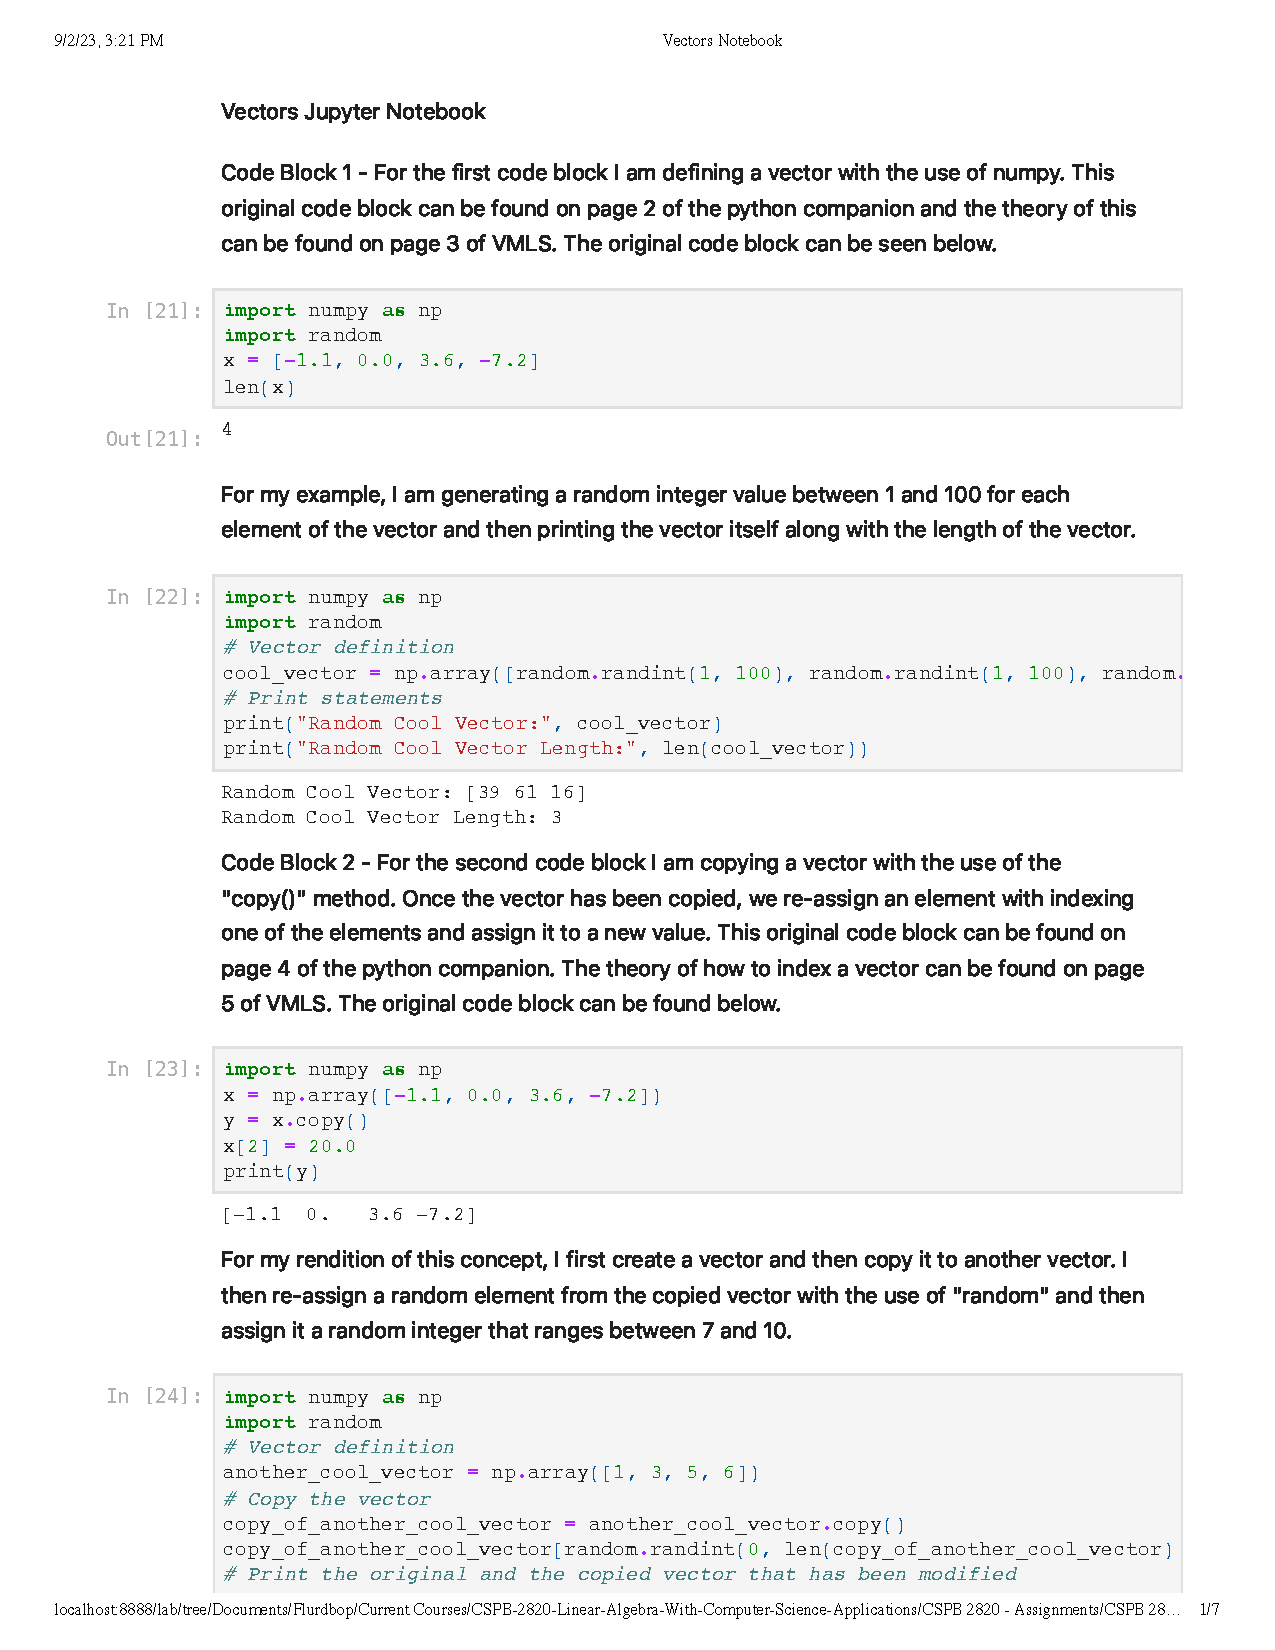
\includepdf[pages={-}, pagecommand={\thispagestyle{fancy}}, width=\paperwidth, offset=0 0]{./PDF/Notebook.pdf}
\end{problem}

% Problem 5 Summary
\begin{summary}{Problem 5 Summary}
    \begin{statement}{Procedure}
        \begin{itemize}
            \item For this problem we showcase different examples from VMLS with the use of a Jupyter notebook
        \end{itemize}
    \end{statement}
    \begin{statement}{Key Concepts}
        \begin{itemize}
            \item This problem showcases many properties of inner products with the use of Jupyter notebook and python
        \end{itemize}
    \end{statement}
    \begin{statement}{Variations}
        \begin{itemize}
            \item We could be asked to copy code from a different section of VMLS
        \end{itemize}
    \end{statement}
\end{summary}

\end{document}
% ----- ----- ----- ----- ----- End Document